\chapter{Fisiologia Vegetal Molecular e Respostas ao Estresse}\label{ch:b3:plant-molecular-physiology}

Uma plântula de feijão crescida num armário escuro é uma coisa pálida e
esguia: um caule longo e branco, um gancho no alto, duas folhas amarelas
dobradas. Leve-a a uma janela e, em um dia, ela parou de se alongar,
endireitou o gancho, abriu e esverdeou as folhas --- um organismo
diferente, a partir dos mesmos genes. Ela não estava esperando energia;
estava esperando informação. Um fóton vermelho absorvido por uma única
proteína lhe diz que chegou à luz; a razão entre o vermelho e o
vermelho-distante lhe diz se há a folha de um vizinho acima; a duração
da noite lhe diz a estação; uma queda do potencial hídrico de suas
raízes, um toque de vento, a flagelina de uma bactéria em sua folha ---
cada um é detectado por um receptor, convertido num sinal químico e
respondido por uma mudança em quais genes são expressos e quais células
crescem. Uma planta não pode fugir de seu ambiente; ela precisa lê-lo e
remodelar a si mesma. Este capítulo trata dessa leitura: os
fotorreceptores, os \omterm{def:b3:endocrinology:hormone}{hormônios} e como eles agem na escala molecular, as
respostas à seca, ao sal, ao frio e ao calor, e o sistema imune de duas
camadas que as plantas desenvolveram sem uma única célula móvel.

\section{Ler a luz}

\begin{definition}[Fotorreceptores]\label{def:b3:plant-molecular-physiology:photoreceptors}
\index{fitocromo}\index{criptocromo}\index{fototropina}\index{fotomorfogênese}\index{estiolamento}
As plantas percebem a luz com três famílias de proteínas, nenhuma delas
a clorofila. Os \emph{fitocromos} são dímeros com um pigmento bilina que
a luz vermelha (\qty{660}{nm}) comuta da forma inativa \emph{Pr} para a
ativa \emph{Pfr}, e de volta pelo vermelho-distante (\qty{730}{nm}); a
Pfr entra no núcleo e marca para degradação uma família de fatores de
transcrição, os PIFs, liberando os genes do desenvolvimento à luz; no
escuro a Pfr reverte devagar. Os \emph{criptocromos} (azul,
\qty{450}{nm}) são flavoproteínas aparentadas a enzimas de reparo do
DNA, que controlam o desestiolamento, o relógio e a floração; as
\emph{fototropinas} (azul) são quinases de membrana que dirigem a
curvatura em direção à luz, a abertura dos estômatos e o movimento dos
cloroplastos. Uma plântula no escuro está \emph{estiolada} --- hipocótilo
longo, cotilédones fechados, nenhuma clorofila, todos os recursos gastos
em alcançar a superfície; a luz a comuta para a \emph{fotomorfogênese}, e
a chave é acionada pela Pfr e pelo criptocromo ao inativarem um único
complexo repressor (COP1) que, no escuro, destrói os fatores de
transcrição do programa de luz. A luz é, portanto, lida duas vezes: como
energia, pelo cloroplasto, e como sinal, por receptores sensíveis a
fluxos de fótons um milhão de vezes menores.
\end{definition}

\begin{proposition}[O fotoequilíbrio do fitocromo]\label{prop:b3:plant-molecular-physiology:photoequilibrium}
\index{fotoequilíbrio}\index{razão vermelho:vermelho-distante}\index{fuga da sombra}
Sob luz contínua a Pr e a Pfr se interconvertem até que as duas taxas de
fotoconversão se equilibrem: com $k_{1}$ a taxa de Pr $\to$ Pfr
(proporcional ao fluxo vermelho) e $k_{2}$ a de Pfr $\to$ Pr
(proporcional ao fluxo vermelho-distante, mais um pouco do vermelho, que
a Pfr também absorve), a fração da forma ativa é
\[
\varphi = \frac{[\text{Pfr}]}{[\text{Pfr}] + [\text{Pr}]} = \frac{k_{1}}{k_{1} + k_{2}},
\]
independente do fluxo total e fixada apenas pela \emph{\omterm{prop:b3:plant-molecular-physiology:photoequilibrium}{razão
vermelho:vermelho-distante}} $\zeta$ da luz. O vermelho puro dá $\varphi \approx 0.87$ (a Pfr absorve também um pouco de vermelho), o
vermelho-distante puro dá $0.03$; a luz do dia aberto, $\zeta \approx
1.15$, dá cerca de $0.55$, e a luz sob um dossel de folhas, cuja
clorofila retirou o vermelho e deixou passar o vermelho-distante, tem
$\zeta \approx 0.2$ e $\varphi \approx 0.2$. Uma planta lê seu $\varphi$
como a presença de vizinhos: um valor baixo dispara a síndrome de
\emph{\omterm{prop:b3:plant-molecular-physiology:photoequilibrium}{fuga da sombra}} --- caules alongados, folhas erguidas, floração
precoce, menos ramificação --- pelos PIFs que a Pfr já não destrói. O
plantio adensado de um agricultor é uma corrida de fugitivos da sombra;
os trigos anões da Revolução Verde, insensíveis ao sinal, puseram no
grão o crescimento poupado.
\end{proposition}
\begin{proof}
$\mathrm{d}[\text{Pfr}]/\mathrm{d}t = k_{1}[\text{Pr}] - k_{2}[\text{Pfr}]$
com $[\text{Pr}] + [\text{Pfr}] = P$ fixo dá, em regime estacionário,
$k_{1}(P - [\text{Pfr}]) = k_{2}[\text{Pfr}]$, donde $\varphi = k_{1}/
(k_{1} + k_{2})$. As duas taxas são proporcionais ao fluxo incidente, de
modo que escalar a luz escala as duas e deixa $\varphi$ inalterado; só a
composição espectral importa. O regime estacionário é atingido com taxa
$k_{1} + k_{2}$ --- segundos sob o sol, minutos ao crepúsculo --- e a
reversão no escuro da Pfr, com meia-vida de horas, fixa o que resta à
noite.
\end{proof}

\begin{omfigure}
\begin{tikzpicture}[every node/.style={font=\scriptsize}, >=stealth]
  \node[draw, very thick, omDef, fill=omDef!15, rounded corners, minimum width=1.6cm, minimum height=0.9cm] (pr) at (0,0) {Pr (inativa)};
  \node[draw, very thick, omThm, fill=omThm!15, rounded corners, minimum width=1.6cm, minimum height=0.9cm] (pfr) at (4.2,0) {Pfr (ativa)};
  \draw[->, very thick, red!70!black] (pr.north east) to[bend left=25] node[above] {vermelho, \qty{660}{nm}} (pfr.north west);
  \draw[->, very thick, red!40!black] (pfr.south west) to[bend left=25] node[below] {vermelho-distante, \qty{730}{nm}} (pr.south east);
  \draw[->, thick, gray] (pfr.south) ++(0.5,-0.15) to[bend left=40] node[right, font=\tiny, gray] {reversão no escuro, horas} ++(-0.3,-0.9);
  \draw[->, thick] (pfr.east) -- ++(1.0,0) node[right, align=left] {para o núcleo:\\PIFs degradados, COP1 desligado;\\programa de luz ligado};
  \begin{scope}[shift={(0,-4.6)}]
  \begin{axis}[
    width=0.55\linewidth, height=4.6cm,
    axis x line=bottom, axis y line=left,
    xmin=0, xmax=2.5, ymin=0, ymax=1,
    xlabel={razão vermelho:vermelho-distante $\zeta$}, ylabel={$\varphi = $ fração Pfr},
    xlabel style={font=\scriptsize, at={(axis description cs:0.5,-0.15)}, anchor=north}, ylabel style={font=\scriptsize},
    tick label style={font=\scriptsize}, xtick={0.2,0.5,1.15,2}, xticklabels={0.2,0.5,1.15,2}, ytick={0.2,0.55,0.87},
    clip=false,
  ]
  \addplot[very thick, omDef, domain=0:2.5, samples=80] {0.87*x/(x+0.6)};
  \draw[dashed, gray] (axis cs:0.2,0) -- (axis cs:0.2,0.22) -- (axis cs:0,0.22);
  \draw[dashed, gray] (axis cs:1.15,0) -- (axis cs:1.15,0.57) -- (axis cs:0,0.57);
  \node[font=\tiny, anchor=west, align=left] at (axis cs:0.25,0.12) {sob um dossel:\\fuga da sombra};
  \node[font=\tiny, anchor=south west] at (axis cs:1.2,0.62) {dia aberto};
  \node[font=\tiny, anchor=north west, omDef, align=left] at (axis cs:1.6,0.45) {um ajuste empírico,\\$\varphi \approx 0.87\,\zeta/(\zeta + 0.6)$};
  \end{axis}
  \end{scope}
\end{tikzpicture}

{\small A chave do \omterm{def:b3:plant-molecular-physiology:photoreceptors}{fitocromo}. A luz vermelha faz a forma ativa, o
vermelho-distante a desfaz, o escuro a reverte devagar; a fração
estacionária da forma ativa depende do equilíbrio de cores da luz, e não
de seu brilho, que é como uma plântula sabe que há uma folha acima dela.}
\end{omfigure}

\begin{proof}[Evidência]
Borthwick, Hendricks e colaboradores (1952) deram a sementes de alface
lampejos breves: o vermelho as fazia germinar, o vermelho-distante dado
em seguida cancelava, o vermelho de novo restaurava, e assim por diante
ao longo de uma dúzia de alternâncias --- o último lampejo decidia, a
assinatura de um pigmento reversível, que eles então extraíram (1959)
como uma proteína azul que mudava seu espectro de absorção sob vermelho
e vermelho-distante. Mostrou-se depois que todo o programa da plântula
crescida no escuro pende de um único repressor: mutantes sem COP1 se
desenvolvem na escuridão total como se estivessem na luz, curtos e
prontos para esverdear, e mutantes deficientes em \omterm{def:b3:plant-molecular-physiology:photoreceptors}{fitocromo} e
\omterm{def:b3:plant-molecular-physiology:photoreceptors}{criptocromo} permanecem estiolados na luz.
\end{proof}

\begin{omfigure}
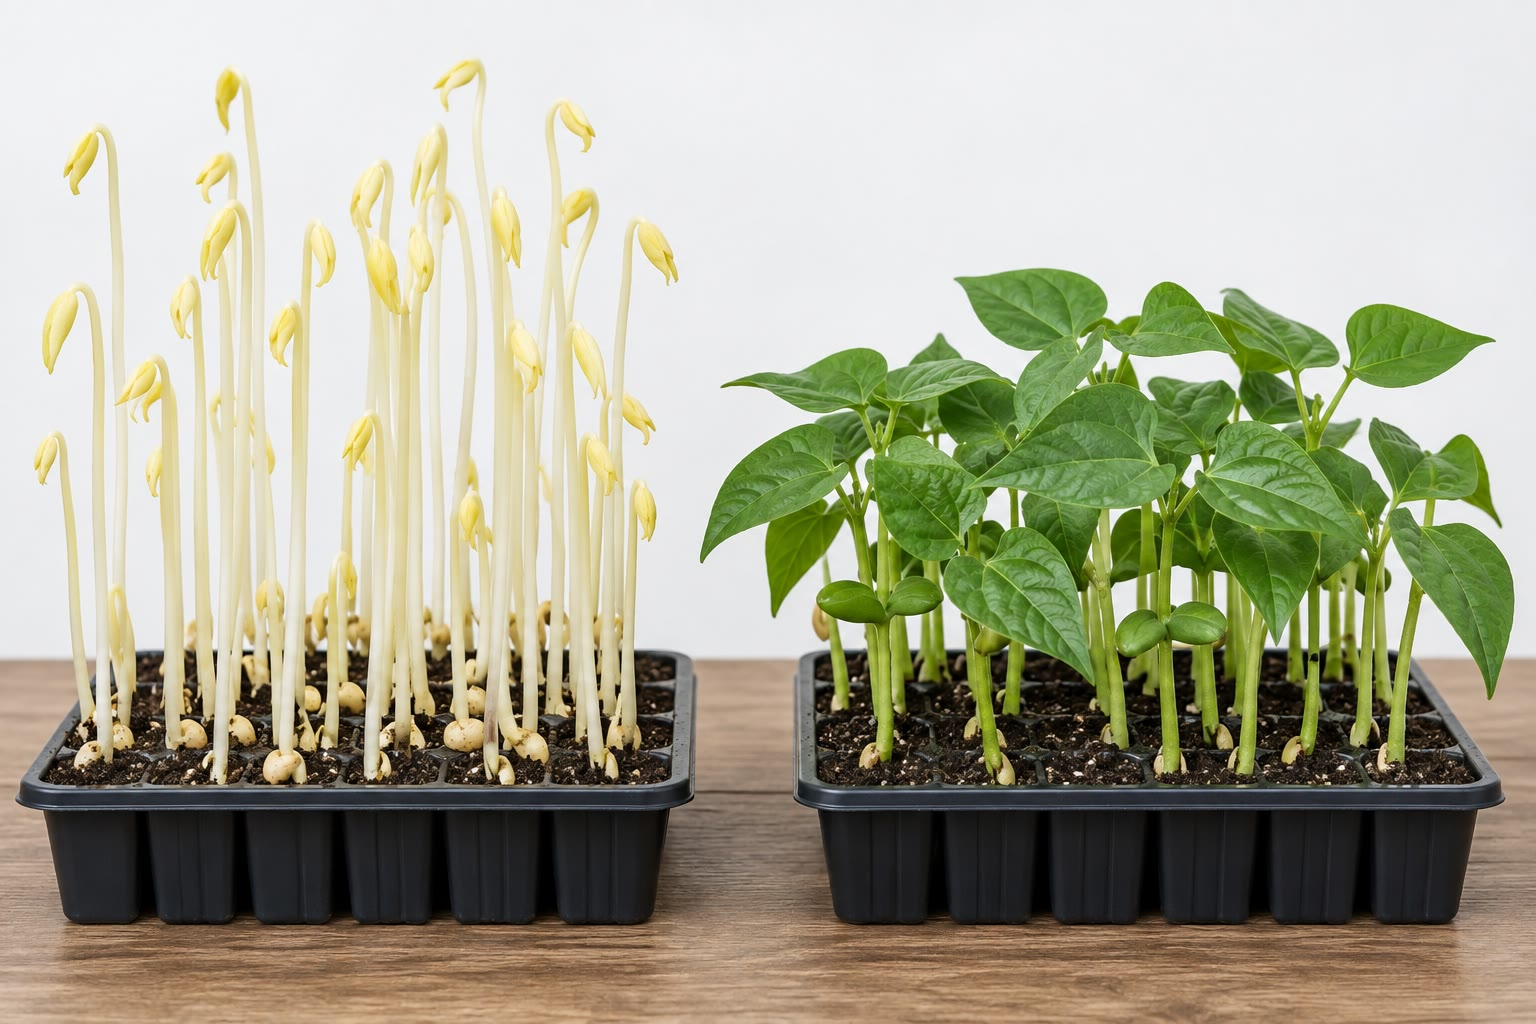
\includegraphics[width=0.56\linewidth]{images/book5/ai/b5-22-etiolated-seedlings.jpg}

{\small Plântulas crescidas no escuro e na luz: o mesmo genoma, dois
programas de desenvolvimento, e a diferença é um único fóton vermelho
absorvido pelo \omterm{def:b3:plant-molecular-physiology:photoreceptors}{fitocromo}.}
\end{omfigure}

\section{Hormônios na escala molecular}

\begin{definition}[Os hormônios vegetais e seus receptores]\label{def:b3:plant-molecular-physiology:hormones}
\index{auxina}\index{TIR1}\index{giberelina}\index{DELLA}\index{ácido abscísico}\index{etileno}\index{citocinina}\index{brassinosteroide}
O volume do Ano~1 descreveu o que os \omterm{def:b3:endocrinology:hormone}{hormônios} vegetais fazem; aqui está
como eles são ouvidos. Vários agem por \emph{destruição regulada}. A
\emph{auxina} (ácido indol-3-acético) liga a proteína F-box \emph{TIR1},
colando-a aos repressores Aux/IAA, que são então ubiquitinados e
destruídos pelo proteassomo: os genes de resposta à auxina que eles
reprimiam ligam em minutos --- o \omterm{def:b3:endocrinology:hormone}{hormônio} é uma cola molecular, e o
receptor faz parte da maquinaria de degradação. A \emph{giberelina} faz o
mesmo com os repressores \emph{DELLA} do crescimento, por seu receptor
GID1: os trigos e arrozes anões da Revolução Verde carregam proteínas
DELLA que não podem ser destruídas e, por isso, permanecem baixos por
mais giberelina que produzam. O \emph{jasmonato} segue a mesma lógica com
os repressores JAZ. O \emph{ácido abscísico} (ABA), o \omterm{def:b3:endocrinology:hormone}{hormônio} da seca e
da dormência, liga os receptores PYR/PYL, que então inibem uma fosfatase
(PP2C), liberando uma quinase (SnRK2) que fosforila canais iônicos e
fatores de transcrição --- uma dupla negação que torna a resposta
íngreme. O \emph{etileno}, um gás, liga receptores contendo cobre na
membrana do RE que, em sua ausência, reprimem ativamente a resposta;
ligá-los os desliga, e os genes de amadurecimento, \omterm{def:b3:cell-cycle-apoptosis:other}{senescência} e estresse
ligam. As \emph{citocininas} agem por receptores histidina-quinase, como
os \omterm{def:b3:bacteriology:quorum}{sistemas de dois componentes} bacterianos; os \emph{brassinosteroides},
os esteroides das plantas, por uma quinase receptora de superfície, e não
por um \omterm{def:b3:endocrinology:hormone}{receptor nuclear} --- os únicos \omterm{def:b3:endocrinology:hormone}{hormônios esteroides} ouvidos, em
qualquer lugar, na superfície celular. As plantas não têm glândulas: cada
\omterm{def:b3:endocrinology:hormone}{hormônio} é feito onde é necessário, ou movido por transportadores
específicos, e sua concentração é fixada localmente por síntese,
conjugação e destruição.
\end{definition}

\begin{theorem}[Transporte polar quimiosmótico da auxina]\label{thm:b3:plant-molecular-physiology:auxin}
\index{transporte polar de auxina}\index{proteínas PIN}\index{aprisionamento do ânion}
O ácido indol-3-acético é um ácido fraco, $\mathrm{p}K_{a} = 4.75$. No
espaço da parede celular, em pH~$5.5$, uma fração substancial é a forma
neutra IAAH, que se difunde através da membrana; no citosol, em pH~$7.2$,
quase tudo é o ânion IAA$^{-}$, que não consegue sair por difusão. No
equilíbrio da forma neutra através da membrana, a razão entre a \omterm{def:b3:plant-molecular-physiology:hormones}{auxina}
total de dentro e a de fora é
\[
\frac{[\text{IAA}]_{\text{in}}}{[\text{IAA}]_{\text{out}}}
= \frac{1 + 10^{\,\mathrm{pH}_{\text{in}} - \mathrm{p}K_{a}}}{1 + 10^{\,\mathrm{pH}_{\text{out}} - \mathrm{p}K_{a}}}
\approx \frac{283}{6.6} \approx 43 :
\]
a célula aprisiona \omterm{def:b3:plant-molecular-physiology:hormones}{auxina} quarenta vezes. Ela só pode sair pelos
transportadores de efluxo \emph{PIN} e, como cada célula põe seus PINs
numa só face --- a face basal, no caule ---, a \omterm{def:b3:plant-molecular-physiology:hormones}{auxina} captada por todos
os lados sai pelo fundo, entra na célula seguinte, e assim por diante:
uma coluna de células com a mesma polaridade é uma esteira que move
\omterm{def:b3:plant-molecular-physiology:hormones}{auxina} a cerca de \qty{1}{cm/h} da ponta do caule à raiz, e reorientar os
PINs redireciona o fluxo, que é como o lado sombreado de um caule passa a
ter mais \omterm{def:b3:plant-molecular-physiology:hormones}{auxina} e a crescer mais depressa.
\end{theorem}
\begin{proof}
Henderson--Hasselbalch: $[\text{IAA}^{-}]/[\text{IAAH}] = 10^{\,\mathrm{pH}
- \mathrm{p}K_{a}}$, de modo que o total $= [\text{IAAH}](1 + 10^{\,\mathrm{pH} -
\mathrm{p}K_{a}})$. A forma neutra se equilibra,
$[\text{IAAH}]_{\text{in}}
= [\text{IAAH}]_{\text{out}}$; dividir os
totais dá a razão, $(1 + 10^{2.45})/(1 + 10^{0.75}) = 283/6.6$. Com os
PINs numa só face, a única saída do ânion é direcional; uma coluna de $n$
células passa o fluxo adiante, e a velocidade medida, uma ordem de
grandeza acima da difusão nessas distâncias, é a do efluxo mediado por
transportador em cada limite celular. A hipótese de Cholodny--Went (anos
1920) de que a curvatura decorre de uma redistribuição lateral de \omterm{def:b3:plant-molecular-physiology:hormones}{auxina}
foi confirmada por medida direta em coleóptilos de aveia e por imagens da
relocação das PIN em raízes de \emph{Arabidopsis} deitadas de lado (anos
2000).
\end{proof}

\begin{omfigure}
\begin{tikzpicture}[every node/.style={font=\scriptsize}, >=stealth]
  % three cells in a column
  \foreach \y in {0,-2.2,-4.4} {
    \draw[thick, omDef, fill=omDef!8] (0,\y) rectangle (3.2,\y-1.9);
    \draw[very thick, omThm] (0.6,\y-1.9) -- (2.6,\y-1.9);
    \node[right, font=\tiny] at (3.3,\y-0.4) {citosol pH 7.2};
    \node[right, font=\tiny] at (3.3,\y-0.8) {IAA$^{-}$ aprisionado};
    \draw[->, thick, omDef!70!black] (-0.6,\y-0.6) -- (0.4,\y-0.6); \node[left, font=\tiny] at (-0.6,\y-0.6) {IAAH entra};
    \draw[->, thick, omDef!70!black] (3.8,\y-1.3) -- (2.8,\y-1.3);
    \draw[->, very thick, omThm] (1.6,\y-1.5) -- (1.6,\y-2.35);
  }
  \node[left, align=right, font=\tiny] at (-0.6,-1.4) {parede pH 5.5:\\\qty{15}{\%} IAAH,\\\qty{85}{\%} IAA$^{-}$};
  \node[omThm, right, font=\tiny] at (3.3,-2.05) {transportadores de efluxo PIN, só na face basal};
  \node[above] at (1.6,0.1) {ponta do caule: fonte de auxina};
  \node[below] at (1.6,-6.8) {rumo à raiz, \qty{1}{cm/h}};
  \node[right, align=left] at (5.4,-3.6) {dentro : fora $\approx 43 : 1$\\(aprisionamento do ânion)\\[3pt]saída só pelos PINs,\\de modo que a coluna é uma esteira;\\mova os PINs para uma face lateral\\e o fluxo vira};
\end{tikzpicture}

{\small O modelo quimiosmótico do \omterm{thm:b3:plant-molecular-physiology:auxin}{transporte polar de auxina}. O ácido
entra por qualquer face como molécula neutra, é aprisionado como ânion no
pH do citosol, e só sai pelos transportadores que a célula colocou numa
face --- de modo que uma fileira de células passa \omterm{def:b3:plant-molecular-physiology:hormones}{auxina} numa só direção.}
\end{omfigure}

\begin{example}[Gravitropismo e fototropismo]\label{ex:b3:plant-molecular-physiology:tropism}
Deite uma plântula de lado. Na coifa da raiz, plastídios densos e cheios
de amido assentam sobre o novo lado inferior das células da columela em
minutos; os transportadores PIN3 dessas células se relocam para a face
inferior; a \omterm{def:b3:plant-molecular-physiology:hormones}{auxina} flui preferencialmente pelo flanco inferior da raiz,
onde, acima do ótimo para as células radiculares, ela \emph{inibe} o
alongamento, e a raiz se curva para baixo. No caule o mesmo fluxo lateral
para o lado inferior \emph{promove} o alongamento (o ótimo das células
caulinares é mais alto), e o caule se curva para cima. Fototropismo: a
\omterm{def:b3:plant-molecular-physiology:photoreceptors}{fototropina} do lado iluminado de um caule altera a colocação das PIN, de
modo que a \omterm{def:b3:plant-molecular-physiology:hormones}{auxina} se acumula no lado sombreado, que cresce mais depressa
e curva o caule em direção à luz. Os dois movimentos são lentos --- horas
--- porque são crescimento, e não movimento, e os dois são irreversíveis
no tecido que já cresceu. Darwin (1880) mostrou que a ponta de uma
plântula de gramínea percebe a luz e a região abaixo se curva; Went
(1928) recolheu a influência num bloco de ágar posto sobre uma ponta
cortada e mostrou que um bloco posto assimetricamente sobre um caule
decapitado o fazia curvar: a influência era uma substância difusível, que
foi então batizada de \omterm{def:b3:plant-molecular-physiology:hormones}{auxina}.
\end{example}

\section{Água, sal, frio e calor}

\begin{definition}[Estresse abiótico]\label{def:b3:plant-molecular-physiology:abiotic}
\index{estresse hídrico}\index{ajuste osmótico}\index{estresse salino}\index{aclimatação ao frio}\index{proteínas de choque térmico}
Uma planta não pode escapar, então ela se endurece. \emph{Seca}: a queda
do potencial hídrico nas raízes dispara a síntese de ABA; o ABA fecha os
estômatos em minutos e, ao longo de dias, liga genes para o \emph{ajuste
osmótico} (prolina, açúcares e outros solutos compatíveis se acumulam,
baixando o potencial hídrico da célula, de modo que ela continue puxando
água), para desidrinas que protegem proteínas, e para uma área foliar
menor e uma raiz mais profunda. O \emph{sal} é seca mais veneno: o sódio
entra por canais de potássio e compete com o potássio; as plantas
tolerantes o bombeiam de volta para fora das raízes (a via SOS), para
dentro de vacúolos (trocadores NHX), ou o excretam por glândulas
foliares, e seu extremo \emph{halófito} vive em água do mar. \emph{Frio}:
o resfriamento enrijece as membranas e retarda as enzimas; o congelamento
puxa a água das células para o gelo extracelular e as desidrata. A
\emph{aclimatação ao frio} --- uma semana de dias frescos --- induz os
fatores de transcrição CBF, que ligam centenas de genes de lipídios que
fluidificam a membrana, açúcares, proteínas anticongelantes e
desidrinas, e um centeio de inverno que morreria a \qty{-5}{\celsius} em
agosto sobrevive a \qty{-30}{\celsius} em janeiro. O \emph{calor}
desenovela proteínas; em minutos após uma elevação, um fator de choque
térmico libera \emph{proteínas de choque térmico}, \omterm{def:b3:structural-biology:chaperones}{chaperonas} que as
reenovelam ou descartam, das mesmas famílias de todo organismo. A
\emph{inundação} priva as raízes de oxigênio; o arroz faz canais de ar
(aerênquima) e se alonga para manter as folhas acima da água, sendo o
\omterm{def:b3:plant-molecular-physiology:hormones}{etileno} o sinal que se acumula quando não consegue escapar para a água.
Muitos desses programas se sobrepõem --- o ABA, as espécies reativas de
oxigênio e os picos de cálcio são segundos mensageiros compartilhados ---
e uma planta aclimatada a um estresse está muitas vezes em parte
protegida contra outro.
\end{definition}

\begin{proposition}[O estômato como válvula]\label{prop:b3:plant-molecular-physiology:stomata}
\index{estômato}\index{célula-guarda}\index{condutância estomática}\index{eficiência do uso da água}
Um par de \emph{células-guarda} delimita cada poro estomático; o poro
abre quando elas captam potássio e ânions (e fazem açúcar), incham e se
arqueiam para os lados, e fecha quando os perdem. A luz azul
(\omterm{def:b3:plant-molecular-physiology:photoreceptors}{fototropinas}), o CO$_{2}$ baixo e a umidade abrem; o escuro, o
CO$_{2}$ alto, a seca e o ABA fecham. A rota do ABA: receptor $\to$
fosfatase inibida $\to$ quinase ativa $\to$ canais de ânions (SLAC1)
abrem $\to$ a membrana despolariza $\to$ o potássio sai por canais de
efluxo $\to$ a água segue $\to$ o poro fecha, em dez minutos. O poro é
onde a troca central da planta é feita: o CO$_{2}$ se difunde para dentro
e o vapor de água para fora pelo mesmo buraco e, como o gradiente de
vapor (uma folha a \qty{100}{\%} de umidade por dentro contra ar a
\qty{50}{\%}) é cinquenta vezes mais íngreme que o gradiente de CO$_{2}$
(\qty{400}{ppm} fora, \qty{250}{} dentro), uma folha perde várias
centenas de moléculas de água por molécula de carbono que fixa. A
\emph{\omterm{prop:b3:plant-molecular-physiology:stomata}{condutância estomática}} $g_{s}$ fixa os dois fluxos: transpiração
$E = g_{s}\,\Delta w$ e assimilação $A = (g_{s}/1.6)\,\Delta c$ (sendo o
CO$_{2}$ mais pesado, difunde-se $1.6$ vez mais devagar), de modo que a
\emph{\omterm{prop:b3:plant-molecular-physiology:stomata}{eficiência do uso da água}} $A/E = \Delta c/(1.6\,\Delta w)$ depende
dos gradientes, e não de quanto o poro está aberto; fechar o poro baixa
os dois fluxos juntos, e elevar o CO$_{2}$ interno (plantas C$_{4}$, que
o concentram) ou abrir apenas à noite (plantas CAM, em ar fresco e úmido)
é como as plantas do deserto melhoram a razão.
\end{proposition}
\begin{proof}
A lei de Fick através do poro para cada gás, com a mesma condutância
geométrica escalada pela razão dos coeficientes de difusão
$D_{\mathrm{H_2O}}/D_{\mathrm{CO_2}} = 1.6$; dividir os dois fluxos
cancela $g_{s}$. Números: $\Delta w \approx \qty{15}{mmol/mol}$ de ar a
\qty{25}{\celsius} e \qty{50}{\%} de umidade, $\Delta c \approx
\qty{150}{\micro mol/mol}$: $A/E = 150/(1.6\times\num{15000}) = 1/160$
--- $160$ moléculas de água por CO$_{2}$ nessas condições amenas, $500$
em ar seco. A sequência de ação do ABA foi desvendada com protoplastos de
células-guarda sob patch clamp, com a corrente de ânions aparecendo em um
minuto após o ABA e o mutante sem SLAC1 falhando em fechar.
\end{proof}

\begin{omfigure}
\begin{tikzpicture}[every node/.style={font=\scriptsize}, >=stealth]
  % pore with two guard cells
  \begin{scope}[shift={(0,0)}]
    \fill[omProp!30] (0,0) ellipse (1.4 and 0.9);
    \fill[white] (0,0) ellipse (0.5 and 0.6);
    \draw[thick, omProp!80!black] (0,0) ellipse (1.4 and 0.9); \draw[thick, omProp!80!black] (0,0) ellipse (0.5 and 0.6);
    \node[below, font=\tiny] at (0,-1.0) {aberto: K$^{+}$, Cl$^{-}$, malato dentro, túrgido};
    \draw[->, thick, omDef] (0,0.3) -- (0,1.5) node[above, font=\tiny] {H$_2$O sai, $E = g_{s}\Delta w$};
    \draw[->, thick, omThm] (0,1.5) ++(-1.0,0) -- ++(0,-1.2); \node[left, font=\tiny, omThm] at (-1.1,1.0) {CO$_2$ entra, $A = g_{s}\Delta c/1.6$};
  \end{scope}
  \begin{scope}[shift={(4.2,0)}]
    \fill[omProp!30] (0,0) ellipse (1.2 and 0.75);
    \draw[thick, omProp!80!black] (0,0) ellipse (1.2 and 0.75); \draw[very thick, omProp!80!black] (0,-0.5) -- (0,0.5);
    \node[below, font=\tiny] at (0,-0.9) {fechado: íons perdidos, flácido};
  \end{scope}
  \draw[->, thick] (1.6,0) -- (2.8,0) node[midway, above, font=\tiny] {ABA, escuro,};
  \node[font=\tiny] at (2.2,-0.25) {CO$_2$ alto};
  % ABA pathway chain
  \begin{scope}[shift={(7.0,1.7)}]
    \node[draw, rounded corners, fill=omDef!20, align=center, font=\tiny] (a) at (0,0) {ABA liga\\PYR/PYL};
    \node[draw, rounded corners, fill=omThm!15, align=center, font=\tiny] (b) at (0,-0.9) {fosfatase PP2C\\inibida};
    \node[draw, rounded corners, fill=omMeth!25, align=center, font=\tiny] (c) at (0,-1.8) {quinase SnRK2\\ativa};
    \node[draw, rounded corners, fill=omProp!25, align=center, font=\tiny] (d) at (0,-2.7) {canal de ânions SLAC1\\aberto: despolarização};
    \node[draw, rounded corners, fill=omProp!25, align=center, font=\tiny] (e) at (0,-3.6) {K$^{+}$ sai, água sai,\\o poro fecha em \qty{10}{min}};
    \draw[-|, thick] (a) -- (b); \draw[-|, thick] (b) -- (c); \draw[->, thick] (c) -- (d); \draw[->, thick] (d) -- (e);
    \node[right, font=\tiny, align=left] at (1.5,-0.9) {duas inibições\\em série:\\uma chave íngreme};
  \end{scope}
\end{tikzpicture}

{\small O estômato e o sinal que o fecha. A água e o gás carbônico
compartilham o poro, de modo que a planta troca um pelo outro a uma taxa
fixada pelos dois gradientes; o \omterm{def:b3:endocrinology:hormone}{hormônio} da seca fecha a válvula por uma
cadeia de duas inibições, o que torna a resposta abrupta.}
\end{omfigure}

\begin{omfigure}
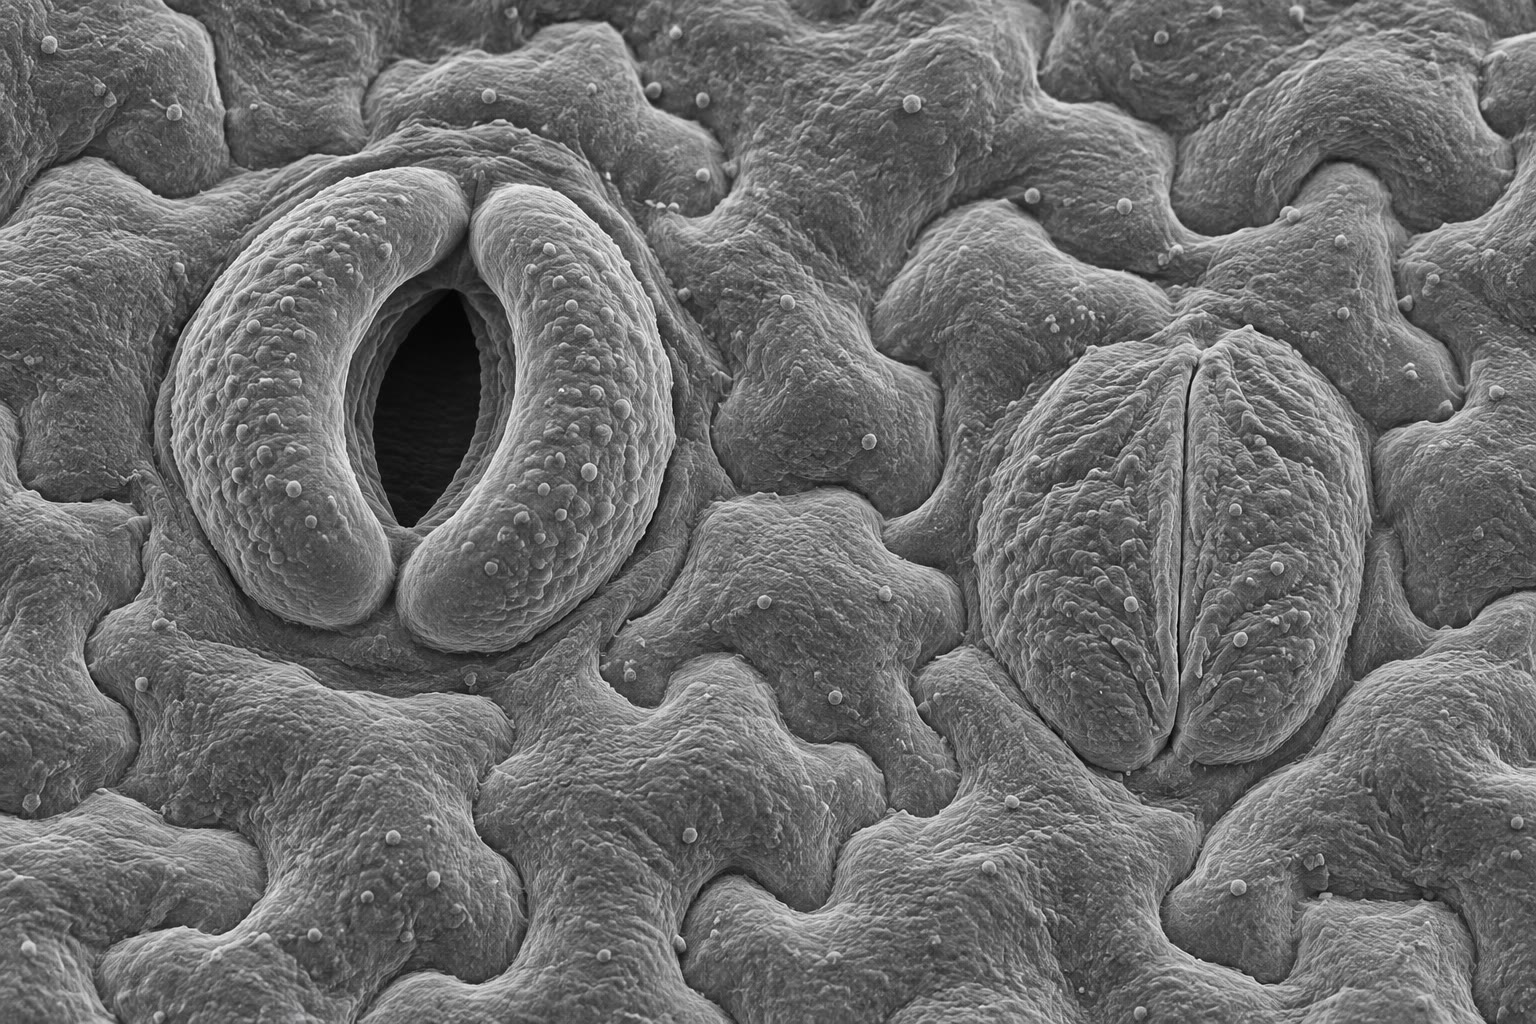
\includegraphics[width=0.46\linewidth]{images/book5/ai/b5-22-stomata-sem.jpg}\hspace{0.04\linewidth}
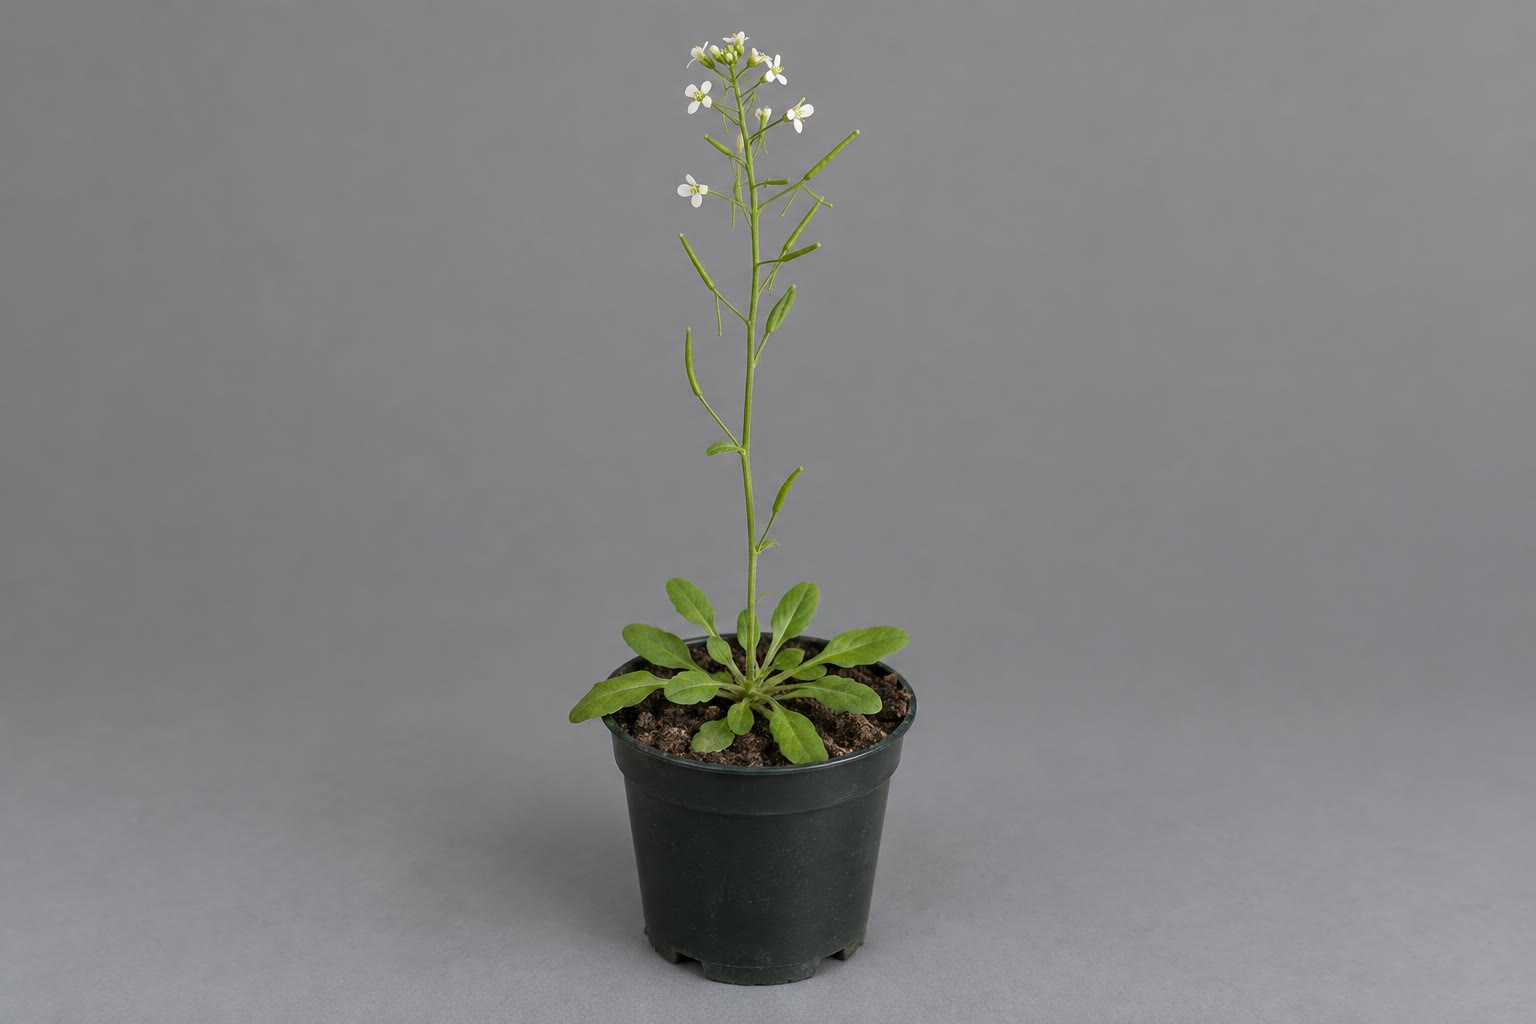
\includegraphics[width=0.46\linewidth]{images/book5/ai/b5-22-arabidopsis.jpg}

{\small À esquerda: estômatos na superfície de uma folha, cada poro entre
suas duas células-guarda, alguns abertos e alguns fechados. À direita:
\emph{Arabidopsis thaliana}, uma erva de beira de estrada com um genoma
pequeno, uma geração de seis semanas e cem mil linhagens mutantes, na
qual a maioria das moléculas deste capítulo foi encontrada.}
\end{omfigure}

\section{Imunidade sem células imunes}

\begin{definition}[Duas camadas da imunidade vegetal]\label{def:b3:plant-molecular-physiology:immunity}
\index{imunidade desencadeada por padrões}\index{imunidade desencadeada por efetores}\index{receptor NLR}\index{resposta hipersensível}\index{resistência sistêmica adquirida}\index{ácido salicílico}\index{ácido jasmônico}
Toda célula vegetal é sua própria célula imune. A primeira camada, a
\emph{imunidade desencadeada por padrões} (PTI), usa quinases receptoras
de superfície que reconhecem moléculas comuns a classes inteiras de
micróbios --- a FLS2 liga um pedaço de 22 aminoácidos da flagelina
bacteriana, outras ligam fragmentos de quitina das paredes fúngicas ---
e, em minutos, lança um influxo de cálcio, uma explosão de oxigênio
reativo, cascatas de quinases, o fechamento dos estômatos, o
espessamento da parede com calose e a transcrição de centenas de genes de
defesa; ela contém a maioria dos micróbios. Os patógenos que vencem
injetam \emph{efetores} --- proteínas que desabilitam componentes da PTI
--- e, contra estes, a segunda camada, a \emph{imunidade desencadeada por
efetores} (ETI), põe em campo \emph{receptores NLR} intracelulares (de
ligação a nucleotídeo e repetições ricas em leucina), cada um
reconhecendo um efetor ou o dano que ele faz, no pareamento gene a gene
que Flor descreveu na ferrugem do linho (anos 1940). A ETI é mais rápida
e mais forte que a PTI e costuma terminar na \emph{resposta
hipersensível}: a célula infectada e suas vizinhas se matam, murando o
patógeno em tecido morto --- as pequenas manchas marrons de uma folha
resistente. As duas camadas liberam \omterm{def:b3:endocrinology:hormone}{hormônios} que levam o alarme: o
\emph{ácido salicílico} contra biotróficos (que se alimentam de células
vivas), disparando a \emph{resistência sistêmica adquirida} por toda a
planta durante semanas; o \emph{ácido jasmônico} e o \omterm{def:b3:plant-molecular-physiology:hormones}{etileno} contra
necrotróficos (que matam e depois se alimentam) e insetos mastigadores,
com jasmonatos voláteis avisando as plantas vizinhas e atraindo os
parasitoides dos insetos. Os dois \omterm{def:b3:endocrinology:hormone}{hormônios} se antagonizam, e alguns
patógenos exploram isso: uma bactéria que fabrica um imitador de
jasmonato desliga a defesa por salicilato que a teria detido.
\end{definition}

\begin{omfigure}
\begin{tikzpicture}
\begin{axis}[
  width=0.78\linewidth, height=5.4cm,
  axis x line=bottom, axis y line=left,
  xmin=0, xmax=10, ymin=0, ymax=10,
  xlabel={a corrida armamentista, da esquerda para a direita}, ylabel={amplitude da defesa},
  xlabel style={font=\small, at={(axis description cs:0.5,-0.08)}, anchor=north}, ylabel style={font=\small},
  xtick=\empty, ytick=\empty,
  clip=false,
]
\addplot[very thick, omDef] coordinates {(0,1) (1.5,5)};
\addplot[very thick, omThm] coordinates {(1.5,5) (3.2,1.8)};
\addplot[very thick, omDef] coordinates {(3.2,1.8) (4.8,8)};
\addplot[very thick, omThm] coordinates {(4.8,8) (6.4,2.2)};
\addplot[very thick, omDef] coordinates {(6.4,2.2) (8.0,8.6)};
\draw[dashed, gray] (axis cs:0,4) -- (axis cs:8.5,4); \node[font=\scriptsize, gray, anchor=west] at (axis cs:8.5,4) {limiar de resistência};
\draw[dashed, gray] (axis cs:0,7.2) -- (axis cs:8.5,7.2); \node[font=\scriptsize, gray, anchor=west] at (axis cs:8.5,7.2) {resposta hipersensível};
\node[font=\scriptsize, omDef, anchor=south west] at (axis cs:0.1,5.3) {PTI: os receptores veem flagelina, quitina};
\node[font=\scriptsize, omThm, anchor=north, align=center] at (axis cs:3.2,1.6) {efetores injetados:\\PTI desabilitada};
\node[font=\scriptsize, omDef, anchor=south, align=center] at (axis cs:4.8,8.2) {ETI: um NLR reconhece\\um efetor};
\node[font=\scriptsize, omThm, anchor=north, align=center] at (axis cs:6.4,2.0) {efetor perdido ou alterado:\\reconhecimento burlado};
\node[font=\scriptsize, omDef, anchor=south, align=center] at (axis cs:8.0,8.8) {um NLR novo\\evolui};
\end{axis}
\end{tikzpicture}

{\small O ziguezague da coevolução planta--patógeno. Receptores de
superfície erguem uma defesa contra moléculas microbianas comuns; os
patógenos injetam efetores que a suprimem; as plantas desenvolvem
receptores intracelulares para os efetores; os patógenos os descartam ou
os alteram; e assim por diante, cada passo deixando genes de resistência
e de virulência que melhoristas e patógenos ainda trocam.}
\end{omfigure}

\begin{proof}[Evidência]
Flor (anos 1940) cruzou variedades de linho e linhagens de ferrugem e
descobriu que a resistência a cada linhagem segregava como um único gene
dominante da planta, pareado com um único gene de avirulência do fungo
--- a relação gene a gene, inexplicada por cinquenta anos, até que os
primeiros genes NLR foram clonados (1994) e se mostrou que os primeiros
pares efetor--receptor se ligavam ou marcavam o dano um do outro.
Gómez-Gómez e Boller (2000) encontraram o mutante de \emph{Arabidopsis}
cego à flagelina, o \emph{fls2}, e mostraram que sua quinase receptora
ligava o peptídeo flg22 em concentração nanomolar e que o mutante era
mais suscetível a bactérias pulverizadas sobre suas folhas, mas não a
bactérias injetadas nelas --- o receptor guarda a superfície e os
estômatos por onde as bactérias entram. Ross (1961) inoculou uma folha de
uma planta de tabaco com um \omterm{def:b3:virology:virus}{vírus} e encontrou as outras folhas
resistentes uma semana depois: a \omterm{def:b3:plant-molecular-physiology:immunity}{resistência sistêmica adquirida}, que
mais tarde se mostrou precisar do \omterm{def:b3:plant-molecular-physiology:immunity}{ácido salicílico}, que a planta faz pela
mesma via que a molécula-mãe da aspirina.
\end{proof}

\begin{example}[O relógio da planta e a duração do dia]\label{ex:b3:plant-molecular-physiology:clock}
As plantas mantêm um \omterm{def:b3:endocrinology:clock}{relógio circadiano} do mesmo desenho que o dos
animais e de peças não aparentadas: fatores da manhã (CCA1, LHY)
reprimem um gene da tarde (TOC1) cujo produto as reprime, com outras
alças que fazem um ciclo robusto de 24 horas mesmo sob luz constante,
antecipando o amanhecer ao abrir os estômatos e ligar os genes da
fotossíntese uma hora antes do sol. A saída mais consequente do relógio é
a medida da duração do dia. Em \emph{Arabidopsis}, uma planta de dia
longo, o relógio faz a proteína CONSTANS se acumular no fim da tarde; num
dia longo essa tarde ainda está iluminada, o \omterm{def:b3:plant-molecular-physiology:photoreceptors}{fitocromo} e o \omterm{def:b3:plant-molecular-physiology:photoreceptors}{criptocromo}
estabilizam a proteína, e ela liga o \emph{FT} na folha; num dia curto a
proteína é feita no escuro e destruída. A proteína FT, o florígeno que os
experimentos de enxertia perseguiam desde Chailakhyan (1936), viaja pelo
floema até o ápice caulinar e, com um parceiro de lá, converte o ápice de
fazer folhas em fazer flores. As plantas de dia curto (arroz, soja) usam
o mesmo relógio com o sinal invertido. Uma planta lê, assim, o calendário
comparando um ritmo interno com a luz externa --- a ``coincidência
externa'' que Bünning propôs em 1936 e que a genética molecular tornou
literal setenta anos depois.
\end{example}

\begin{remark}[Ficar parado, mudar tudo]\label{rem:b3:plant-molecular-physiology:remark}
A resposta do animal a um ambiente ruim é deixá-lo; a da planta é tornar-se
uma planta diferente. Ela tem receptores para a cor e a direção da luz,
para o puxão da gravidade, para o potencial hídrico de seu solo, para o
toque do vento e para a química de seus inimigos; seus \omterm{def:b3:endocrinology:hormone}{hormônios} agem
destruindo repressores, de modo que um sinal pode comutar um programa em
minutos; e cada uma de suas células é seu próprio sensor, seu próprio
sistema imune e, se preciso, seu próprio meristema regenerador. Os trigos
anões que alimentaram um mundo em crescimento foram uma proteína \omterm{def:b3:plant-molecular-physiology:hormones}{DELLA}
que não podia ser degradada; as culturas tolerantes à seca das próximas
décadas serão, em boa parte, uma questão de receptores de ABA,
\omterm{prop:b3:plant-molecular-physiology:stomata}{condutância estomática} e a \omterm{prop:b3:plant-molecular-physiology:stomata}{eficiência do uso da água} que este capítulo
calculou.
\end{remark}

\section{Exercícios}

\begin{exercise}[$\star$]\label{exo:b3:plant-molecular-physiology:1}
Liste as três famílias de fotorreceptores com seus comprimentos de onda
e uma resposta de cada uma. Por que uma planta precisa de
fotorreceptores se já tem clorofila?
\end{exercise}

\begin{exercise}[$\star$]\label{exo:b3:plant-molecular-physiology:2}
Explique como a \omterm{def:b3:plant-molecular-physiology:hormones}{auxina}, a \omterm{def:b3:plant-molecular-physiology:hormones}{giberelina} e o jasmonato compartilham um
mecanismo de ação, e por que isso torna a resposta rápida.
\end{exercise}

\begin{exercise}[$\star$]\label{exo:b3:plant-molecular-physiology:3}
Descreva a sequência de eventos desde a chegada do ABA a uma
célula-guarda até o fechamento do poro, e nomeie o ponto em que uma
mutação deixaria a planta incapaz de fechar seus estômatos.
\end{exercise}

\begin{exercise}[$\star$]\label{exo:b3:plant-molecular-physiology:4}
Distinga a \omterm{def:b3:plant-molecular-physiology:immunity}{imunidade desencadeada por padrões} da desencadeada por
efetores pelo que é reconhecido, onde está o receptor e como a resposta
termina.
\end{exercise}

\begin{exercise}[$\star\star$]\label{exo:b3:plant-molecular-physiology:5}
Usando o ajuste $\varphi \approx 0.87\,\zeta/(\zeta + 0.6)$, calcule a
fração de Pfr à luz do dia ($\zeta = 1.15$), sob uma folha ($\zeta =
0.4$), sob um dossel denso ($\zeta = 0.1$) e sob uma lâmpada
incandescente ($\zeta = 0.7$). Por que as plântulas sob tais lâmpadas
crescem altas?
\end{exercise}

\begin{exercise}[$\star\star$]\label{exo:b3:plant-molecular-physiology:6}
Calcule a razão dentro:fora para a \omterm{def:b3:plant-molecular-physiology:hormones}{auxina} se o pH da parede for $5.0$ e
o do citosol $7.5$; depois, se a parede for acidificada a $4.5$ (como
fazem as células em crescimento). O que acontece com o aprisionamento se
o citosol acidificar a $6.5$ sob anoxia?
\end{exercise}

\begin{exercise}[$\star\star$]\label{exo:b3:plant-molecular-physiology:7}
A \omterm{def:b3:plant-molecular-physiology:hormones}{auxina} se move a \qty{1}{cm/h} por células de \qty{50}{\micro m} de
comprimento. Quantas células ela cruza por hora, e quanto tempo passa em
cada uma? Compare com o tempo de difundir \qty{50}{\micro m} ($D =
\qty{5e-10}{m^2/s}$, $t \approx x^{2}/2D$) e diga que etapa limita o
transporte.
\end{exercise}

\begin{exercise}[$\star\star$]\label{exo:b3:plant-molecular-physiology:8}
Uma folha a \qty{25}{\celsius} tem uma fração molar interna de vapor de
\qty{32}{mmol/mol} e o ar, \qty{16}{mmol/mol}; o CO$_{2}$ é
\qty{400}{ppm} fora e \qty{250}{ppm} dentro. Calcule as moléculas de água
perdidas por CO$_{2}$ fixado. Recalcule para uma planta C$_{4}$ com
CO$_{2}$ interno a \qty{150}{ppm}, e para um dia seco com o ar a
\qty{8}{mmol/mol}.
\end{exercise}

\begin{exercise}[$\star\star$]\label{exo:b3:plant-molecular-physiology:9}
Explique por que uma planta aclimatada ao frio é muitas vezes também
mais tolerante à seca, nomeando os sinais compartilhados e as moléculas
protetoras compartilhadas.
\end{exercise}

\begin{exercise}[$\star\star\star$]\label{exo:b3:plant-molecular-physiology:10}
O \omterm{def:b3:plant-molecular-physiology:photoreceptors}{fitocromo} se aproxima de seu fotoequilíbrio com taxa $k_{1} + k_{2}$
proporcional ao fluxo. Se o sol pleno dá $k_{1} + k_{2} =
\qty{0.5}{s^{-1}}$, quanto tempo leva a comutação no \qty{1}{\%} do sol
pleno do amanhecer? A Pfr reverte no escuro com meia-vida de
\qty{2}{h}: que fração resta depois de uma noite de 8 horas, e como isso
permite a uma semente distinguir uma exposição breve de um dia?
\end{exercise}

\begin{exercise}[$\star\star\star$]\label{exo:b3:plant-molecular-physiology:11}
A \omterm{def:b3:plant-molecular-physiology:immunity}{resposta hipersensível} mata talvez uma centena de células por sítio de
infecção. Argumente, com uma estimativa grosseira de custo e benefício
para uma folha de $10^{7}$ células diante de dez infecções por dia, por
que o suicídio das células infectadas é barato, e por que um necrotrófico
(que se alimenta de células mortas) transforma essa defesa numa fraqueza.
\end{exercise}

\begin{exercise}[$\star\star\star$]\label{exo:b3:plant-molecular-physiology:12}
Modele a coincidência externa: a proteína CONSTANS é feita entre as horas
12 e 16 depois do amanhecer e destruída com meia-vida de \qty{30}{min} no
escuro, mas de \qty{4}{h} na luz. Estime a proteína restante na hora 16
num dia de 16 horas e num dia de 10 horas (escuro a partir da hora 10), e
explique como um limiar converte isso numa decisão de florescer.
\end{exercise}

\section{Problema: Uma Plântula na Sombra}

\begin{problem}[{Problema de fim de semana --- uma plântula lida por suas
moléculas: o equilíbrio do fitocromo sob um dossel, a auxina que ela
aprisiona e transporta, a água que ela troca por carbono pelos estômatos
e o custo de defender suas folhas, terminando na fração de Pfr sob o
dossel, na razão de aprisionamento da auxina e na eficiência do uso da
água}]
\label{pb:b3:plant-molecular-physiology:1}
Dados: ajuste do fotoequilíbrio $\varphi = 0.87\,\zeta/(\zeta + 0.6)$;
luz do dia $\zeta = 1.15$, dossel $\zeta = 0.2$; taxa de alongamento do
hipocótilo $r = r_{0}(1 - \varphi)$ com $r_{0} = \qty{2}{mm/h}$. \omterm{def:b3:plant-molecular-physiology:hormones}{Auxina}:
$\mathrm{p}K_{a} = 4.75$; pH da parede $5.5$, pH do citosol $7.2$;
velocidade de transporte \qty{1}{cm/h}; comprimento celular
\qty{100}{\micro m}. Folha: fração molar de vapor interna
\qty{32}{mmol/mol}, ar \qty{16}{mmol/mol}; CO$_{2}$ \qty{400}{ppm} fora,
\qty{250}{ppm} dentro; $g_{s} =
\qty{0.3}{mol\,m^{-2}\,s^{-1}}$ (vapor de
água); área foliar \qty{20}{cm^2}; \qty{12}{h} de luz. Defesa: a \omterm{def:b3:plant-molecular-physiology:immunity}{resposta
hipersensível} mata $100$ células por sítio; a folha tem $10^{7}$ células;
a PTI custa \qty{5}{\%} da fotossíntese enquanto está ativa.

\medskip
\noindent\textbf{Parte I --- Luz.}
\begin{enumerate}
  \item Calcule $\varphi$ à luz do dia e sob o dossel.
  \item Taxas de alongamento em cada caso, e o comprimento extra depois
        de \qty{48}{h} na sombra.
  \item A folha de um vizinho remove \qty{90}{\%} do vermelho e
        \qty{20}{\%} do vermelho-distante da luz do dia. Calcule o novo
        $\zeta$ e o novo $\varphi$. Uma única folha basta para disparar a
        \omterm{prop:b3:plant-molecular-physiology:photoequilibrium}{fuga da sombra}?
  \item Explique por que $\varphi$ independe do brilho, e o que isso
        significa para uma plântula num dia nublado a céu aberto.
  \item O sol pleno dá $k_{1} + k_{2} = \qty{0.5}{s^{-1}}$. Tempo para
        alcançar \qty{95}{\%} do fotoequilíbrio no sol pleno e em
        \qty{1}{\%} dele?
  \item A Pfr feita durante o dia reverte com meia-vida de \qty{2}{h}.
        Fração restante depois de \qty{8}{h} e depois de \qty{14}{h} de
        escuro; como uma planta poderia usar isso como relógio da duração
        da noite, e por que ele é um relógio ruim?
\end{enumerate}

\medskip
\noindent\textbf{Parte II --- \omterm{def:b3:plant-molecular-physiology:hormones}{Auxina}.}
\begin{enumerate}[resume]
  \item Fração da \omterm{def:b3:plant-molecular-physiology:hormones}{auxina} que é IAAH neutro na parede e no citosol.
  \item Razão dentro:fora no equilíbrio do IAAH. Se a parede contém
        \qty{0.1}{\micro M} de \omterm{def:b3:plant-molecular-physiology:hormones}{auxina} total, qual é a concentração
        citosólica?
  \item Células cruzadas por hora, e tempo de permanência por célula.
  \item Um caule de \qty{5}{cm}: quanto tempo para uma mudança de \omterm{def:b3:plant-molecular-physiology:hormones}{auxina}
        na ponta chegar à base? Compare com a hora que um caule leva para
        começar a se curvar em direção à luz, e comente.
  \item Numa raiz gravi-estimulada, a PIN3 se reloca de modo que o flanco
        inferior recebe \qty{60}{\%} do fluxo e o superior \qty{40}{\%}.
        Se o alongamento das células radiculares cai \qty{1}{\%} para
        cada \qty{1}{\%} de \omterm{def:b3:plant-molecular-physiology:hormones}{auxina} acima da norma e sobe na mesma medida
        abaixo dela, calcule as taxas dos dois flancos em relação à norma
        e o sentido da curvatura.
  \item Por que a mesma assimetria curva um caule no sentido contrário?
\end{enumerate}

\medskip
\noindent\textbf{Parte III --- Água por carbono.}
\begin{enumerate}[resume]
  \item Transpiração $E = g_{s}\,\Delta w$ em \unit{mmol\,m^{-2}\,s^{-1}}.
  \item Assimilação $A = (g_{s}/1.6)\,\Delta c$ em \unit{\micro
        mol\,m^{-2}\,s^{-1}}, e a razão $E/A$.
  \item Água perdida pela folha de \qty{20}{cm^2} no dia de 12 horas, em
        moles e em gramas; carbono fixado, em moles de CO$_{2}$ e em
        gramas de glicose.
  \item O ABA fecha os estômatos até $g_{s} = \qty{0.05}{}$. Novos $E$ e
        $A$, e a razão. O que a planta ganhou e o que perdeu?
  \item Uma planta C$_{4}$ mantém o CO$_{2}$ interno a \qty{150}{ppm} com
        o mesmo $g_{s}$: seu $E/A$? Uma planta CAM abre à noite, quando
        $\Delta w = \qty{5}{mmol/mol}$: seu $E/A$ com $\Delta c =
        \qty{150}{ppm}$?
  \item Explique por que a razão $E/A$ não depende de $g_{s}$, e o que
        uma planta pode e não pode fazer a respeito.
\end{enumerate}

\medskip
\noindent\textbf{Parte IV --- Defesa.}
\begin{enumerate}[resume]
  \item Dez sítios de infecção por dia, cada um respondido por uma
        \omterm{def:b3:plant-molecular-physiology:immunity}{resposta hipersensível}: células mortas por dia, como fração da
        folha.
  \item Ao longo dos 60 dias de vida de uma folha, que fração é
        sacrificada? Compare com a perda se uma infecção em cada dez
        escapasse e destruísse \qty{5}{\%} da folha a cada vez.
  \item A PTI fica ativa \qty{20}{\%} do tempo: custo médio como fração
        da fotossíntese. Por que as plantas não a mantêm sempre ligada?
  \item Um patógeno deleta o efetor que um NLR reconhece. O que ele
        ganha, o que ele perde, e o que a população de plantas faz em
        seguida?
  \item Uma bactéria secreta um imitador de jasmonato. Que defesa ela
        desliga e por que isso a ajuda, dado o antagonismo entre as duas
        vias hormonais?
  \item Por que uma resistência gene a gene numa lavoura em monocultura
        costuma ser vencida em poucas safras, e o que o ziguezague sugere
        que os melhoristas façam em seu lugar?
  \item Resuma: o $\varphi$ sob o dossel (questão~1), a razão de
        aprisionamento da \omterm{def:b3:plant-molecular-physiology:hormones}{auxina} (questão~8) e as moléculas de água
        perdidas por CO$_{2}$ fixado (questão~14).
\end{enumerate}
\end{problem}
